\chapter{Testing}

%Detailed descriptions of every test case are definitely not what is required here. What is important is to show that you adopted a sensible strategy that was, in principle, capable of testing the system adequately even if you did not have the time to test the system fully.

%Have you tested your system on �real users�? For example, if your system is supposed to solve a problem for a business, then it would be appropriate to present your approach to involve the users in the testing process and to record the results that you obtained. Depending on the level of detail, it is likely that you would put any detailed results in an appendix.

%The following sections indicate some areas you might include. Other sections may be more appropriate to your project.

This chapter discusses the testing strategy which has been implemented on the project. This includes unit, acceptance and user testing utilised throughout various parts of the application.

\section{Overall approach to testing}
To recap, an agile approach was adopted throughout the project. From the process, test-driven-development was used throughout the application for almost all aspects of testing.

\subsection{Test-driven-development}
Test-driven-development (TDD) aims to produce tests prior to the implementation of features. As a result, all implementation code is supported by a series of tests. Figure \ref{fig:tdd} shows the TDD cycle.

\begin{figure}
  \includegraphics[scale=0.5]{images/tdd}
  \centering
  \caption{The cycle of TDD during the development stages of the application}
  \label{fig:tdd}
\end{figure}

Initially a test is created, this would then fail due to no implementation code. The following steps would be to ensure that the tests pass by adding the associated code needed to make sure that it passes. Afterwards refactoring occurs to ensure that design is kept simple and as clean as possible for the current implementation.

With TDD it could have gone one of two ways: a group of tests were created for a feature, or one test for one bit of functionality. The latter approach was chosen, ensuring that the design was carefully considered.

Using TDD allows for the domain of the problem to be considered before implementing code to solve the issue. The user-stories were deconstructed into a series of tasks. There tasks were then formulated into different tests (unit, integration and acceptance). The cycle was then repeated.
\section{Automated testing}
One thing to note is that Flask's testing documentation is very sparse and is of low quality.

During the first few sprints of testing, pytest \cite{citeulike:14020583} was originally being used to create test classes, with test classes sub-classing  \lstinline[basicstyle=\normalsize\ttfamily]{unittest.TestCase}.

Flask tests were refactored mid-way through a series of sprints to use Flask-testing \cite{citeulike:14020588}. This offers better testing support for Flask application, allowing the creation of a fake application and providing the functionality to run a live server for testing, which would be needed for acceptance tests.

\section{Mocking tests}
The purpose of mocking is to change the output of a function to a value which is returned every time \cite{citeulike:14020596}. It was established that certain tests would need to be mocked, because some data would change from test to test. It was identified that \textit{all} interactions with Google API's, any interactions with Tesseract and the Session would need to be mocked.

As discussed by Mathew Dale \cite{citeulike:14020597} when writing tests, mocks are needed because of external factors out of a developer's control. As the Google API does not support specific environment API's, such as production or development, then all URLs would be to a production URL. The issue this raises when testing is ensuring that the tests are isolated and pass every time. For example, the test could query the API once and pass the test, however on the next query it may fail due to a different return value; this requires  mocks to be used. The mock would return a specific value every time, ensuring consistency among tests.

The principle is the same for testing Tesseract in the web application. If more training was conducted then the results from the test on the image would change, therefore the data was mocked from the returned text functions to provide consistency.

During the first few sprints, whilst understanding how mocks work with Python, there was a lot of duplication with the mocking services. The library mock \cite{citeulike:14020599} uses annotations above test functions to signal a mock value.

\begin{lstlisting}[language=python, caption={An example of using mocks, following the annotation pattern}, label={lst:mock1}, breaklines, columns=fullflexible, keywordstyle=\color{blue}, basicstyle=\normalsize\ttfamily]
  @mock.object(GoogleOauthService, 'authorise')
  @mock.object(GoogleCalendarService, 'execute_request')
  def test_return_correct_response(self, authorise, calendar_response):
    authorise.return_value = some_json
    calendar_response.return_value = some_more_json
\end{lstlisting}

In code example \ref{lst:mock1} shows the syntax which was initially used in the tests, for mocking. This would result in many of the tests becoming unreadable obfuscated. Additionally the do not repeat yourself (DRY) principle was violated, by duplicating much of the codebase.

\begin{lstlisting}[language=python, label={lst:mock2}, breaklines, columns=fullflexible, keywordstyle=\color{blue}, label={Mocks using the patch and start. It stops in the dear downs}, basicstyle=\normalsize\ttfamily]
    def setUp(self):
        # some code
        authorise_patch = mock.patch()
        authorise_mock = authorise_patch.start()
        authorise_mock.return_value = some_json


    def tearDown(self):
        mock.patch.stopAll()
\end{lstlisting}
Investigating the mock API documentation, patching object calls was discovered. Implementing this solution reduced the amount of code for mocking specific functions. The annotations were removed from the top of function tests. Initially it was not entirely clear how to implement these patch functions. Eventually the patch was included in the \lstinline[basicstyle=\normalsize\ttfamily]{setUp} and \lstinline[basicstyle=\normalsize\ttfamily]{tearDown} functions, as shown in example \ref{lst:mock2}.


Often when testing there needed to be way to alternate the output of a function. In the Python mock library side effects allowed the mock object to return different values.

\begin{lstlisting}[language=python, label={lst:mock3}, breaklines, columns=fullflexible, keywordstyle=\color{blue}, basicstyle=\normalsize\ttfamily]
    def setUp(self):
        # some code
        self.google_patch = mock.patch.object(GoogleCalendarService, "execute_request")
        self.google_mock = self.google_patch.start()
        self.google_mock.side_effect = [self.google_response, self.new_event, self.google_response, self.updated_response]

    def tearDown(self):
        mock.patch.stopAll()
\end{lstlisting}

Figure \ref{lst:mock3} shows the use of the ``side effect'' API. From the above example, it outputs Google response first, then when \lstinline[basicstyle=\normalsize\ttfamily]{execute_request} is called for a second time \lstinline[basicstyle=\normalsize\ttfamily]{new_event} response is fired and so on. Examples of mocking data can be found in Appendix \ref{appendix:test_data}. An example usage of this would be for when the Google Calendar needed to get a user's events. Firstly, in the controller it would get a list of events and then it would get a singular event. Since the same function call was used, a test needed to be added to check the return values were indeed correct.

Overall, mocking produced a substantial amount of the testing. It was not considered when designing the system that mocking would be needed, it was only when testing happened that it was realised it was needed. The tests were refactored to incorporate the mocking facilities.

\subsection{Unit testing}
A unit test is used for models where functions can be tested in isolation to ensure that they perform the correct operations. In the application unit tests were created for every model.

Sometimes there was a cross over between database transactions and testing specific functions. In these cases, using the actual database would not be used for testing as this would interfere with the actual data in the system.

The config was overwritten to include a test SQLite database. This ensured that a test database was used, which was cleared and created for every test. This allowed each test to be tested independently of one another.

Very much like the function names of the classes, the test cases were as descriptive as possible. This formed part of the documentation of the application.

\begin{figure}[h!]
  \centering
  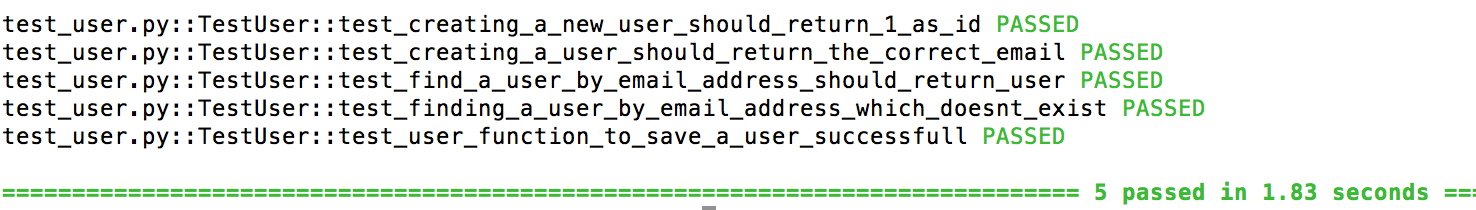
\includegraphics[width=\textwidth]{images/unit_test_user}
  \caption{Example Unit test for the user class. Each of the tests pass}
  \label{fig:unit_user}
\end{figure}

Figure \ref{fig:unit_user} shows an example of the unit tests for the user class. The functions were decomposed and tests were associated for each function. In cases both edge-cases and normal expected results were selected.

Refer to appendix x for full unit test cases.

\subsection{Integration testing}
Due to the application having external routes, then testing them to ensure the correct response codes was important. These were the first tests written for the routing sections, and implemented from the design considerations in section \ref{section:design}.

The tests consisted of checking that the response codes were correct, any redirects were correctly redirected; this tested to ensure the application flow was implemented correctly.

Where there was interactions with the database in the routes, then tests were conducted to ensure the routes performed the correct persistence. For example, when posting to the meta-data URL, then checks were created to ensure that the module code was being persisted correctly.

Appendix \ref{appendix:test_results} section \ref{appendix:integration_tests} depicts the integration tests in the system.

\subsection{Handling sessions}
One of the trickier aspects of testing was the handling of sessions. In parts of the application sessions are used to handle specific states of the system, i.e when a user's logged in.

During testing, sections of the system are tested in isolated environments. If the route to show all the notes was tested, it would require the user to be logged in - therefore storing data in the session. However, when testing this there will be no session set when running the test. Flask had a solution to testing the session handling \cite{citeulike:14020609}.

\begin{lstlisting}[language=python, label={lst:session}, breaklines, columns=fullflexible, keywordstyle=\color{blue}, basicstyle=\normalsize\ttfamily, caption= {An example of how sessions were handled and modified in the tests.}]
  with self.client.session_transaction() as session:
          session['user_id'] = self.user_id
\end{lstlisting}

Figure \ref{lst:session}, displays an example on how the session had to be modified in the integration tests. After the session transaction context has exited then the session has been modified for that test.

Acceptance testing initially proved to be problematic. When testing with the sessions, the selenium tests would not acknowledge that a session had been set, like in Figure \ref{lst:session}, causing the tests to fail. After a lot of problems, it was confirmed that the session helper would have to be mocked, in the \lstinline[basicstyle=\normalsize\ttfamily]{create_app} function, which is initialised when a test is created.

Overall, session handling was one of the hardest aspects with testing to overcome to provide working tests.

\section{Acceptance testing}
Acceptance tests evaluate the system as a whole. This includes testing to ensure that the front-end functionality is what is expected when the user views the web-page.

To implement these tests a tool would be needed to check what the application looked like on a web-page, the tool selected was selenium for Python \cite{citeulike:14020625}. It can integrate with the DOM (document object model), and perform automated browser testing.

When testing with selenium there is the option to test with a standard browser, Chrome, Firefox etc, or it can be tested on a headless browser (via PhantomJS). A headless browser can access a webpage the same as Chrome, but it does not display a graphical user-interface \cite{citeulike:13983611}.

An example of an acceptance test may follow a pattern like:
\begin{enumerate}
  \item Go to page /search.
  \item Find the search field.
  \item Enter the text ``CS31310''
  \item Click submit
  \item Find ``searched-item'' from the DOM.
  \item Return whether it equals ``CS31310''
\end{enumerate}

The above example shows that unlike other tests, which test the specific feature or functionality, this test checks what is displayed to the user via interactions with the web browser. The test then passes or fails based on assertions. Another example of the selenium tests being useful was checking the output colour from Tesseract. The logic in the view file determined the colour and Selenium was able to confirm the logic was correct.

\begin{figure}[h!]
  \centering
  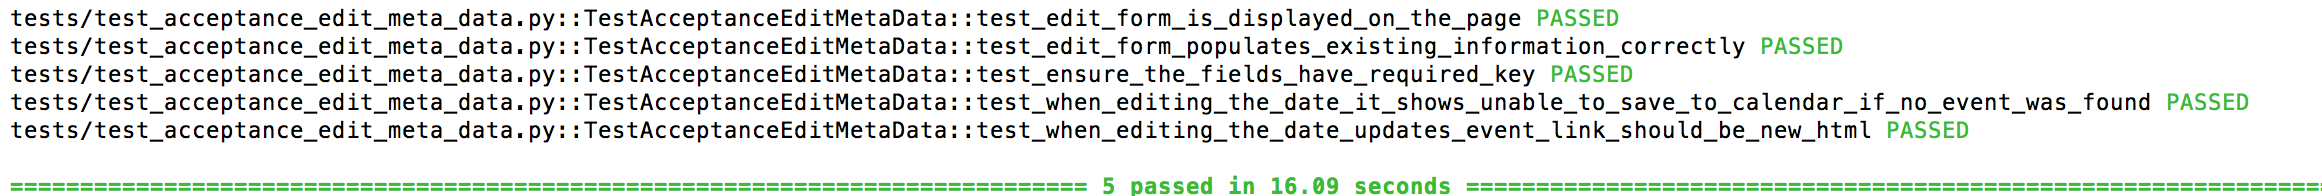
\includegraphics[width=\textwidth]{images/acceptance_test_1}
  \caption{An example of the acceptance tests running. It shows that the time to run the tests have increased considerably.}
  \label{fig:acceptance_test_1}
\end{figure}

In Figure \ref{fig:acceptance_test_1} it shows that the time to run to run 5 tests increased to 16.09 seconds; one of the disadvantages is the time taken to run the test-suite. Due to the complexity with loading data correctly to the view file, then these tests are imperative to ensure the user expects to see the correct content. For full acceptance tests refer to Appendix \ref{appendix:test_results}, section \ref{appendix:acceptance}.

With acceptance tests the classes all subclass the \lstinline[basicstyle=\normalsize\ttfamily]{LiveServerClass} from the Flask-Testing package. This is different than the Integration and Unit tests as they use \lstinline[basicstyle=\normalsize\ttfamily]{TestClass}. The LiveServerClass allows an instance of the application to be loaded alongside selenium, removing the need for an external selenium server or for the tests to be ran with the server running. It was at this time in the sprints which a large refactor of the system occurred, accommodating for the automatic application launch. 

\section{User Testing}
Due to the application aiming to solve a problem, a set of potential user's were asked to perform a user study of the application. Their responses were analysed and their opinions on whether the software met their aims was collated.

Prior to the actual scheduled user-testing, feedback was given regarding the displaying of the Tesseract output confidence. These ``over the shoulder'' comments were along the lines of: ``It would be great if you could click the identified text and it would automatically populate the text boxes''. This was then implemented as a result from pre-user testing.

Further issues which were identified during the user testing were:
\begin{itemize}
  \item Uploading a JPG image off a phone, which does not have the correct date-time exif-data key causes the application to fail.
  \item Uploading an image with a previously uploaded filename caused the application to display the old file.
\end{itemize}

These issues were caught and modified thanks to extensive user-testing of the application.

\begin{figure}[h!]
  \centering
  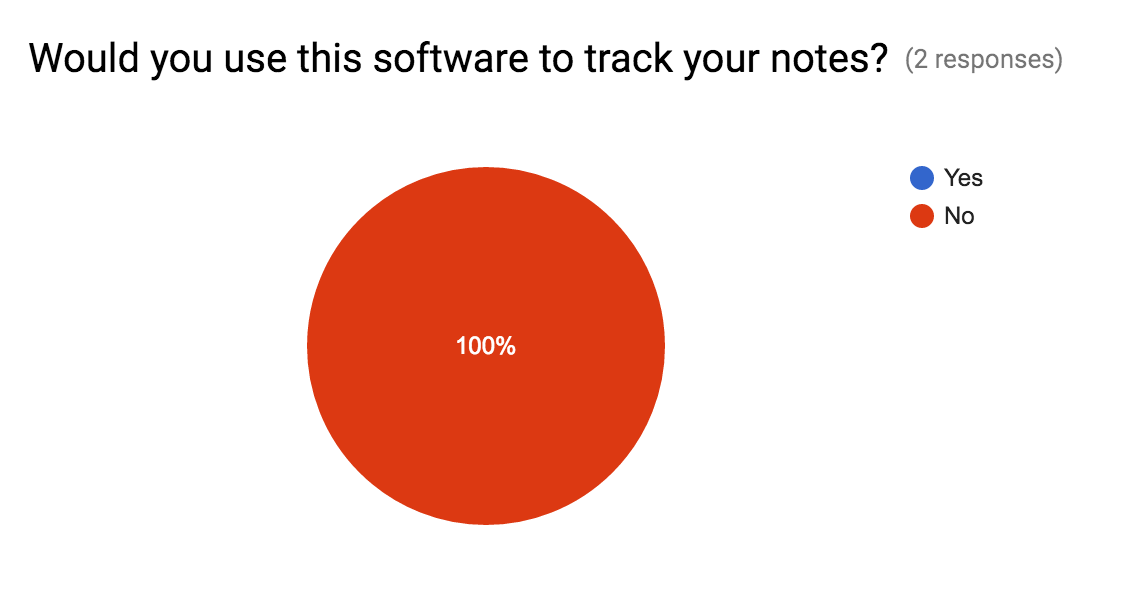
\includegraphics[scale=0.5]{images/user_response}
  \caption{A pie chart from the Google forms questionnaire that the users conducted showing that they would not use the application for archiving their notes.}
  \label{fig:user_response}
\end{figure}

One interesting reflection of the user-case study was that people would not use the application, as shown in Figure \ref{fig:user_response}. They were quick to defend the applications quality, but the use-case for them taking notes was not present. They much preferred to write up their notes from the lecture for memory retention.

\section{Tesseract Testing}
Due to there being no code written for the Tesseract training process there were no formal tests conducted for this section. However, what could be tested was how well the Tesseract learnt as it progressed through the training process.

\begin{figure}[h!]
  \centering
  \includegraphics[scale=0.6]{images/tesseract_testing}
  \caption{A simple framework showing the steps of analysing each of the training examples for a statistical measure for how successful the training process was.}
  \label{fig:tesseract_framework}
\end{figure}

Figure \ref{fig:tesseract_framework} shows a simple framework for analysing how well Tesseract trained the data. After the statistics has been collated then a graph was constructed to show the trends.

\begin{figure}[h!]
  \centering
\begin{tikzpicture}
\begin{axis}[
    title={Tesseract Training examples compared to their success rate of characters identified vs correct characters},
    title style={text width=\textwidth, align=center},
    xlabel={Training example},
    ylabel={Success rate (\%) },
    xmin=0, xmax=100,
    ymin=0, xmax = 100,
    ytick={0,20,40,60,80,100},
    xtick={0, 9,18,27,36,45,54,63, 72, 81 , 90 , 99},
    xticklabels={1, 2, 3, 4, 5, 6, 7, 8, 9 , 10 , 11 ,12 },
    legend pos=north west,
    ymajorgrids=true,
    grid style=dashed,
]

\addplot[
    color=black,
    mark=square,
    ]
    coordinates {
    (0, 61.4035087719298)(9, 72.2222222222222)(18, 81.1594202898551) (27, 79.1044776119403)(36, 69.7916666666667)(45, 74.6376811594203) (54, 78.5276073619632)(63, 69.75)(72, 78.7878787878788)(81, 66.3341645885287)(90, 65.5737704918033)(99, 75.414364640884)
    };

\addplot [thick, red] table[y={create col/linear regression}]{
    0 61.4035087719298
    9 72.2222222222222
    18 81.1594202898551
    27 79.1044776119403
    36 69.7916666666667
    45 74.6376811594203
    54 78.5276073619632
    63 69.75
    72 78.7878787878788
    81 66.3341645885287
    90 65.5737704918033
    99 75.414364640884
    };
\end{axis}
\end{tikzpicture}
\caption{A line-graph showing the success rate of the Tesseract training results over 12 examples.}
\label{fig:tesseract_graph}
\end{figure}

Figure \ref{fig:tesseract_graph} shows the output analysed from the Tesseract training. It shows each training example with an associated success rate for the characters identified. The conclusions clearly show that there is no improvement from the Tesseract output after around the 3rd example. A horizontal linear regression line shows that it has peaked at around 72\% correct recognition rate. Refer to appendix \ref{appendix:tesseract}, section \ref{appendix:tesseract_table} for the full statistics.

\section{Image threshold Testing}
Due to the nature of the image processing script it was quickly realised a methodical approach to testing would not be beneficial, due to almost constant spike work.

TDD would not be performed before considering the design for the image bininarsation script. Instead the testing would consist of a more visual check of the outputted image to see if the result was successfully binarised. Once the script had been developed to a reasonable level of satisfaction the spike work would cease, and testing would ensue.

The code was re-written following a TDD approach. It involved analysing numpy arrays returned from OpenCV and checking, for instance, if any of the array contained black values.

ADD reference to appendix to show examples of output
